\begin{figure}[bth!]
	\begin{center}
		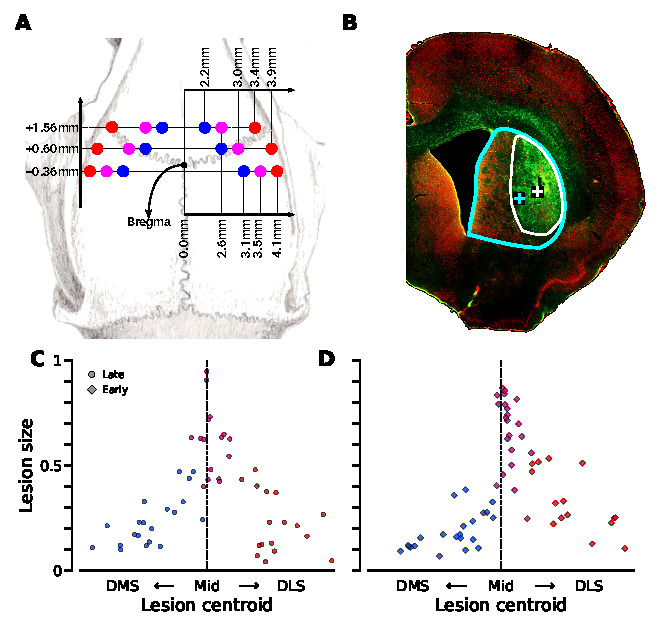
\includegraphics[scale=1]{ch-methods/figures/LesionSizeLocation.pdf}
		\caption[Lesion Coordinates and Quantification]
		{\textbf{Dorsal striatum lesion coordinates and quantification.}
		\textbf{A)} Schematic of lesion sites.
		\textbf{B)} Illustration of the quantification of the lesion size.
		For each coronal slide and hemi-striatum, the contour of the lesion was manually outlined using the GFAP staining.
		The relative size of the lesion (compared to the full striatum, manually outlined on the NeuN staining) and the coordinates of the lesion/striatum centroid was calculated.
		For each animal, the size and location were obtained by averaging data along the anteroposterior axis, for both left and right hemispheres.
		\textbf{C,~D)} Lesion size vs.\ location for animals that underwent lesion before (\textit{C}: early) and after (\textit{D}: late) extensive practice.
		Lesion quantification was performed blindly relative to the behavior.
		In four animals with a striatal lesion performed after learning the task (late lesion), the lesion size quantification could not be properly performed.
		These animals were classified according to their injection coordinates in the surgery (3~DLS, and 1~DMS), however they were excluded from any analysis that required the lesion size (hence the difference between the number of `late lesion' animals in this figure, $n=53$, and the total number of animals in \autoref{fig:lesion:task}, $n=57$).
		}
		\label{fig:method:LesionSizeLocation}
	\end{center}
\end{figure}